\documentclass[12pt]{extarticle}
\usepackage {mathtext}
\usepackage [russian] {babel}
\usepackage {amsmath, caption, geometry, amssymb, graphicx, wrapfig, subfig, derivative}

\captionsetup[table]{
	justification=raggedleft,
	singlelinecheck=false,
	labelsep=colon
}
\newcommand{\eds}{\mathcal{E}}

\geometry{left = 2cm, right=1cm, top=15mm, bottom=20mm}

\title{Лабораторная работа №3.5.1. \\ \textbf{Изучение плазмы газового разряда в неоне}}
\author{Данила Шеломанов, Павел Рудачихин. Б04-507}
\date{27.10.2026}
\begin {document}
\maketitle{}


\section {Аннотация} 
	
	\hspace{4.5mm} Целью настоящей работы является получение вольт-амперной характеристики тлеющего разряда и зондовых характеристик при разных токах заряда; измерение концентрации и температуры электронов, степени ионизации, плазменной частоты и дебаевского радиуса.
	
	В основе экспериментального метода лежит использование двойного зонда для измерения параметров плазмы и снятие вольт-амперной характеристики как двойного зонда, так и самого разряда.

\section{Теоретическое введение}

\hspace{4.5mm} Главные свойства плазмы --- коллективный характер её движения и квазинейтральность. Плазмой называют ионизованный газ, дебаевский радиус которого существенно меньше характерного размера занимаемой им области. Стационарное состояние плазмы возможно лишь при наличии непрерывно действующего источника энергии (в данной работе --- электрического разряда в газе).

\subsection{Дебаевский радиус и плазменная частота}

\hspace{4.5mm} Важнейшими пространственным и временным масштабами плазмы являются дебаевский радиус и плазменная частота. Плазменная (ленгмюровская) частота
\begin{equation}
	\omega_p = \sqrt{\frac{4\pi n e^2}{m_e}}
	\label{eq:omega_p}
\end{equation}
определяет характерное время отклика плазмы на флуктуацию плотности заряда и, в частности, условие распространения электромагнитных волн: волны с $\omega > \omega_p$ проходят через плазму, а с $\omega < \omega_p$ --- отражаются.

В неравновесной плазме, где температуры электронов и ионов различны ($T_e \neq T_i$), вводят два характерных масштаба экранирования. Электронная поляризационная длина (электронный дебаевский радиус)
\begin{equation}
	r_{De} = \sqrt{\frac{kT_e}{4\pi n_e e^2}}
	\label{eq:rDe}
\end{equation}
задаёт масштаб, на котором тепловые флуктуации электронов способны нарушить квазинейтральность, и именно она фигурирует в критерии квазинейтральности плазмы: характерный размер плазмы $L$ должен удовлетворять условию $L \gg r_{De}$.

Полный (эффективный) дебаевский радиус экранирования, учитывающий вклад как электронов, так и ионов, равен
\begin{equation}
	r_D = \left(r_{De}^{-2} + r_{Di}^{-2}\right)^{-1/2}
	= \sqrt{\frac{k}{4\pi n_e e^2}\cdot\frac{T_e T_i}{T_e + T_i}},
	\qquad
	r_{Di} = \sqrt{\frac{kT_i}{4\pi n_i e^2}}.
	\label{eq:rD}
\end{equation}
Именно $r_D$ определяет масштаб, на котором экранируется поле стороннего заряда (например, зонда), помещённого в плазму. В тлеющем разряде $T_e \gg T_i$, поэтому $r_{De} \gg r_{Di}$ и
\begin{equation}
	r_D \approx r_{Di} = \sqrt{\frac{kT_i}{4\pi n_e e^2}},
	\label{eq:rD_limit}
\end{equation}
то есть экранирование поля зонда определяется холодными ионами, тогда как масштаб тепловых флуктуаций электронов задаётся $r_{De}$.

Число частиц в дебаевской сфере
\begin{equation}
	N_D = \frac{4}{3}\pi n r_D^3
	\label{eq:ND}
\end{equation}
характеризует идеальность плазмы: при $N_D \gg 1$ энергия кулоновского взаимодействия частиц мала по сравнению с тепловой, и плазму можно рассматривать как идеальный газ.

Степень ионизации плазмы определяется как доля ионизованных атомов:
\begin{equation}
	\alpha = \frac{N_i}{N} = \frac{n}{n_0} = \frac{n kT}{P},
	\label{eq:alpha}
\end{equation}
где $n_0$ --- полная концентрация частиц, $P$ --- давление газа.

\subsection{Двойной зонд}

\hspace{4.5mm} Двойной зонд --- система из двух одинаковых электродов с малой площадью поверхности $S$, расположенных на небольшом расстоянии $l$ друг от друга. Между зондами создаётся разность потенциалов $U$, много меньшая плавающего потенциала, так что оба зонда находятся на ионной ветви вольт-амперной характеристики.

\begin{figure}[h!]
	\centering
	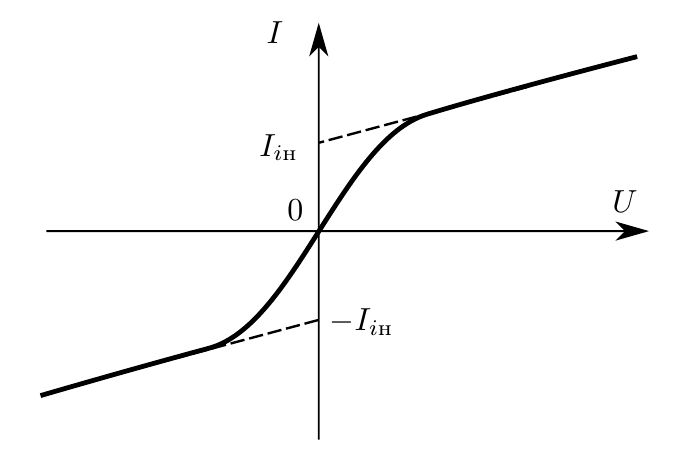
\includegraphics[width=0.5\linewidth]{zond}
	\caption{Типичная ВАХ двойного зонда}
	\label{fig:zond}
\end{figure}


Типичная вольт-амперная характеристика двойного зонда представлена на рис. \ref{fig:zond}. Ток насыщения $I_н$ находится по пересечению асимптот ВАХ с осью $U = 0$. Температуру электронов $T_e$ можно определить по току насыщения и наклону ВАХ вблизи начала координат $dI/dU|_{U=0}$:
\begin{equation}
	kT_e = \frac{1}{2} \frac{eI_н}{\odv{I}{U}|_{U=0}},
	\qquad
	T_e(\text{эВ}) = \frac{1}{2} \frac{I_н}{\odv{I}{U}|_{U=0}}.
	\label{eq:Te}
\end{equation}
Формула следует из теоретической ВАХ двойного зонда $I = I_н \operatorname{th}\dfrac{eU}{2kT_e}$ при разложении вблизи $U=0$.

По полуэмпирической формуле Д. Бома можно определить концентрацию заряженных частиц $n = n_i = n_e$:
\begin{equation}
	I_н = 0{,}4\, n e S \sqrt{\frac{2kT_e}{m_i}}
	\quad\Rightarrow\quad
	n = \frac{I_н}{0{,}4\, e S} \sqrt{\frac{m_i}{2kT_e}}
	= \frac{I_н}{0{,}4\, e S} \sqrt{\frac{\mu}{2RT_e}},
	\label{eq:bohm}
\end{equation}
где $\mu$ --- молярная масса иона, $R = 8{,}31$ Дж/(моль$\cdot$К) --- универсальная газовая постоянная, $m_i$ --- масса иона..

	
\section{Описание установки}

	\hspace{4.5mm} В работе используются: стеклянная газоразрядная трубка с неоном, высоковольтный источник питания, источник питания постоянного тока, делитель напряжения, потенциометр, амперметры, вольтметры, переключатели.
	
	\begin{figure}[h!]
		\centering
		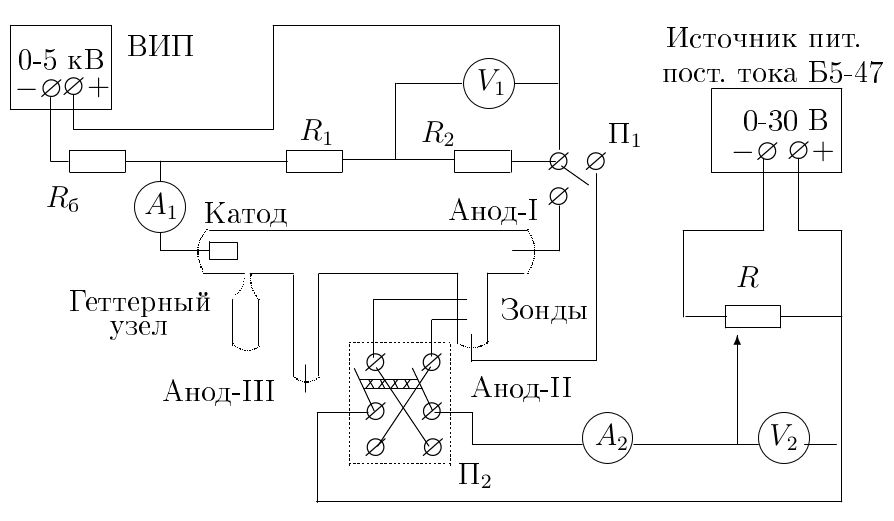
\includegraphics[width=0.7\linewidth]{setup}
		\caption{Схема установки}
		\label{fig:setup}
	\end{figure}
	
	Схема установки приведена на рис. \ref{fig:setup}. Стеклянная газоразрядная трубка имеет не нагреваемый полый катод, три анода и геттерный (газопоглощающий) узел. Трубка заполнена изотопом неона $^{22}Ne$. при давлении 2 мм. рт. ст. Катод и один из анодов I или II с помощью переключателя П$_1$ подключается через балластный резистор $R_б$ к высоковольтному источнику питания (ВИП). 
	
	С помощью амперметра $A_1$ и вольтметра $V_1$ снимается вольт-амперная характеристика газового разряда при переключении П$_1$ на Анод-I, а с помощью $A_2$ и $V_2$ -- двойного зонда при подключении на Анод-II. Переключатель П$_2$ позволяет менять полярность напряжения на зондах. Анод III не используется. 
	
	Параметры зонда: диаметр d = 0,2 мм, длина l = 5,2 мм. Площадь поверхности $S \approx 3,26 \ мм^2$.
	
	
	
\section{Результаты и обсуждения}

	\subsection{ВАХ тлеющего разряда}
	
		\hspace{4mm} Путём плавного увеличения напряжения на ВИП определено напряжение зажигания разряда
		
		\[ U_{заж} = 2040 \ В \]
		
		\begin{figure}[h!]
			\centering
			\subfloat[Экспериментальная]{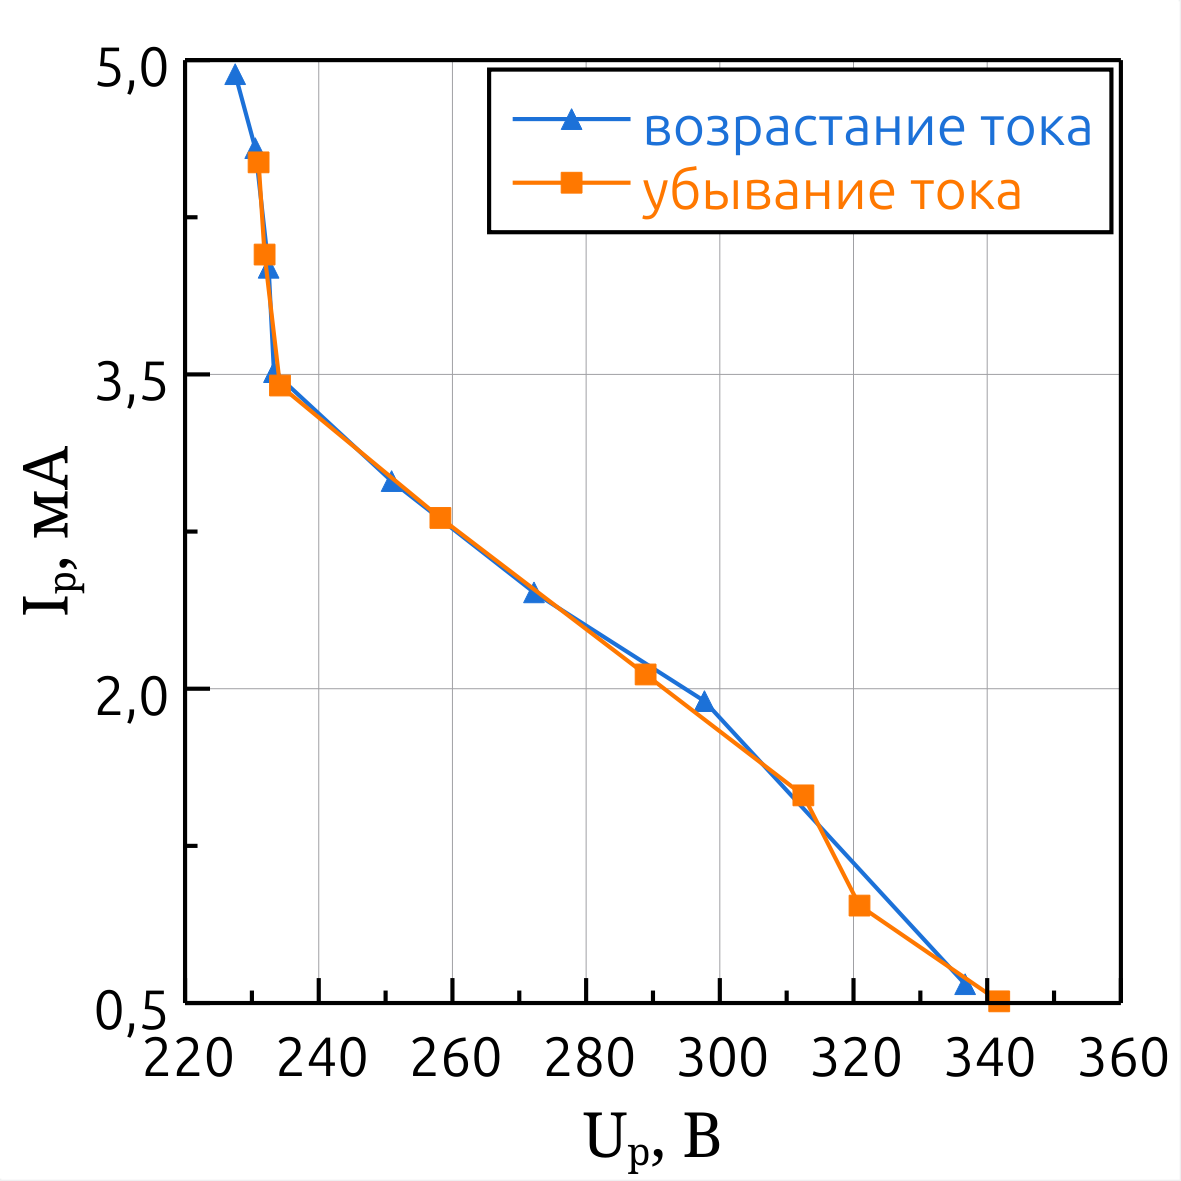
\includegraphics[width=0.5\textwidth]{IpUp}}
			\subfloat[Справочная]{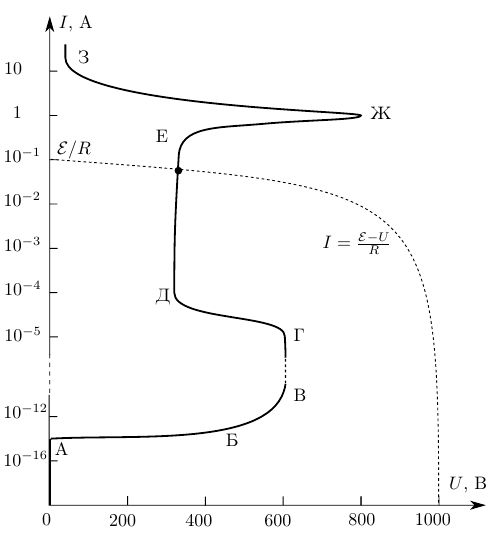
\includegraphics[width=0.4\textwidth]{lab}}
			\caption{ВАХ тлеющего разряда}
			\label{fig:IpUp}\label{fig:lab}
		\end{figure}
		После зажигания напряжение снижается. Вольт-амперная характеристика (ВАХ) тлеющего разряда получена в диапазоне напряжений 227 -- 336 В (см. рис. \ref{fig:IpUp}a). Она имеет отрицательный наклон и заметно изменяет его при напряжении 234 В.
		Исходя из этого, полученная ВАХ соответствует участку Г-Д на рис. \ref{fig:lab}b, причём ближе к точке Д. Этот участок соответстует переходу от поднормального тлеющего разряда к нормальному тлеющему разряду. 
		
		Дифференцированием найдены предельные значения дифференциального сопротивления
		
		\[ R_{min} = -65,8 \ кОм \ \ \ R_{max} = -6,6 \ кОм\]
		
		\subsection{ВАХ двойного зонда}
		
		\begin{figure}[h!]
			\centering
			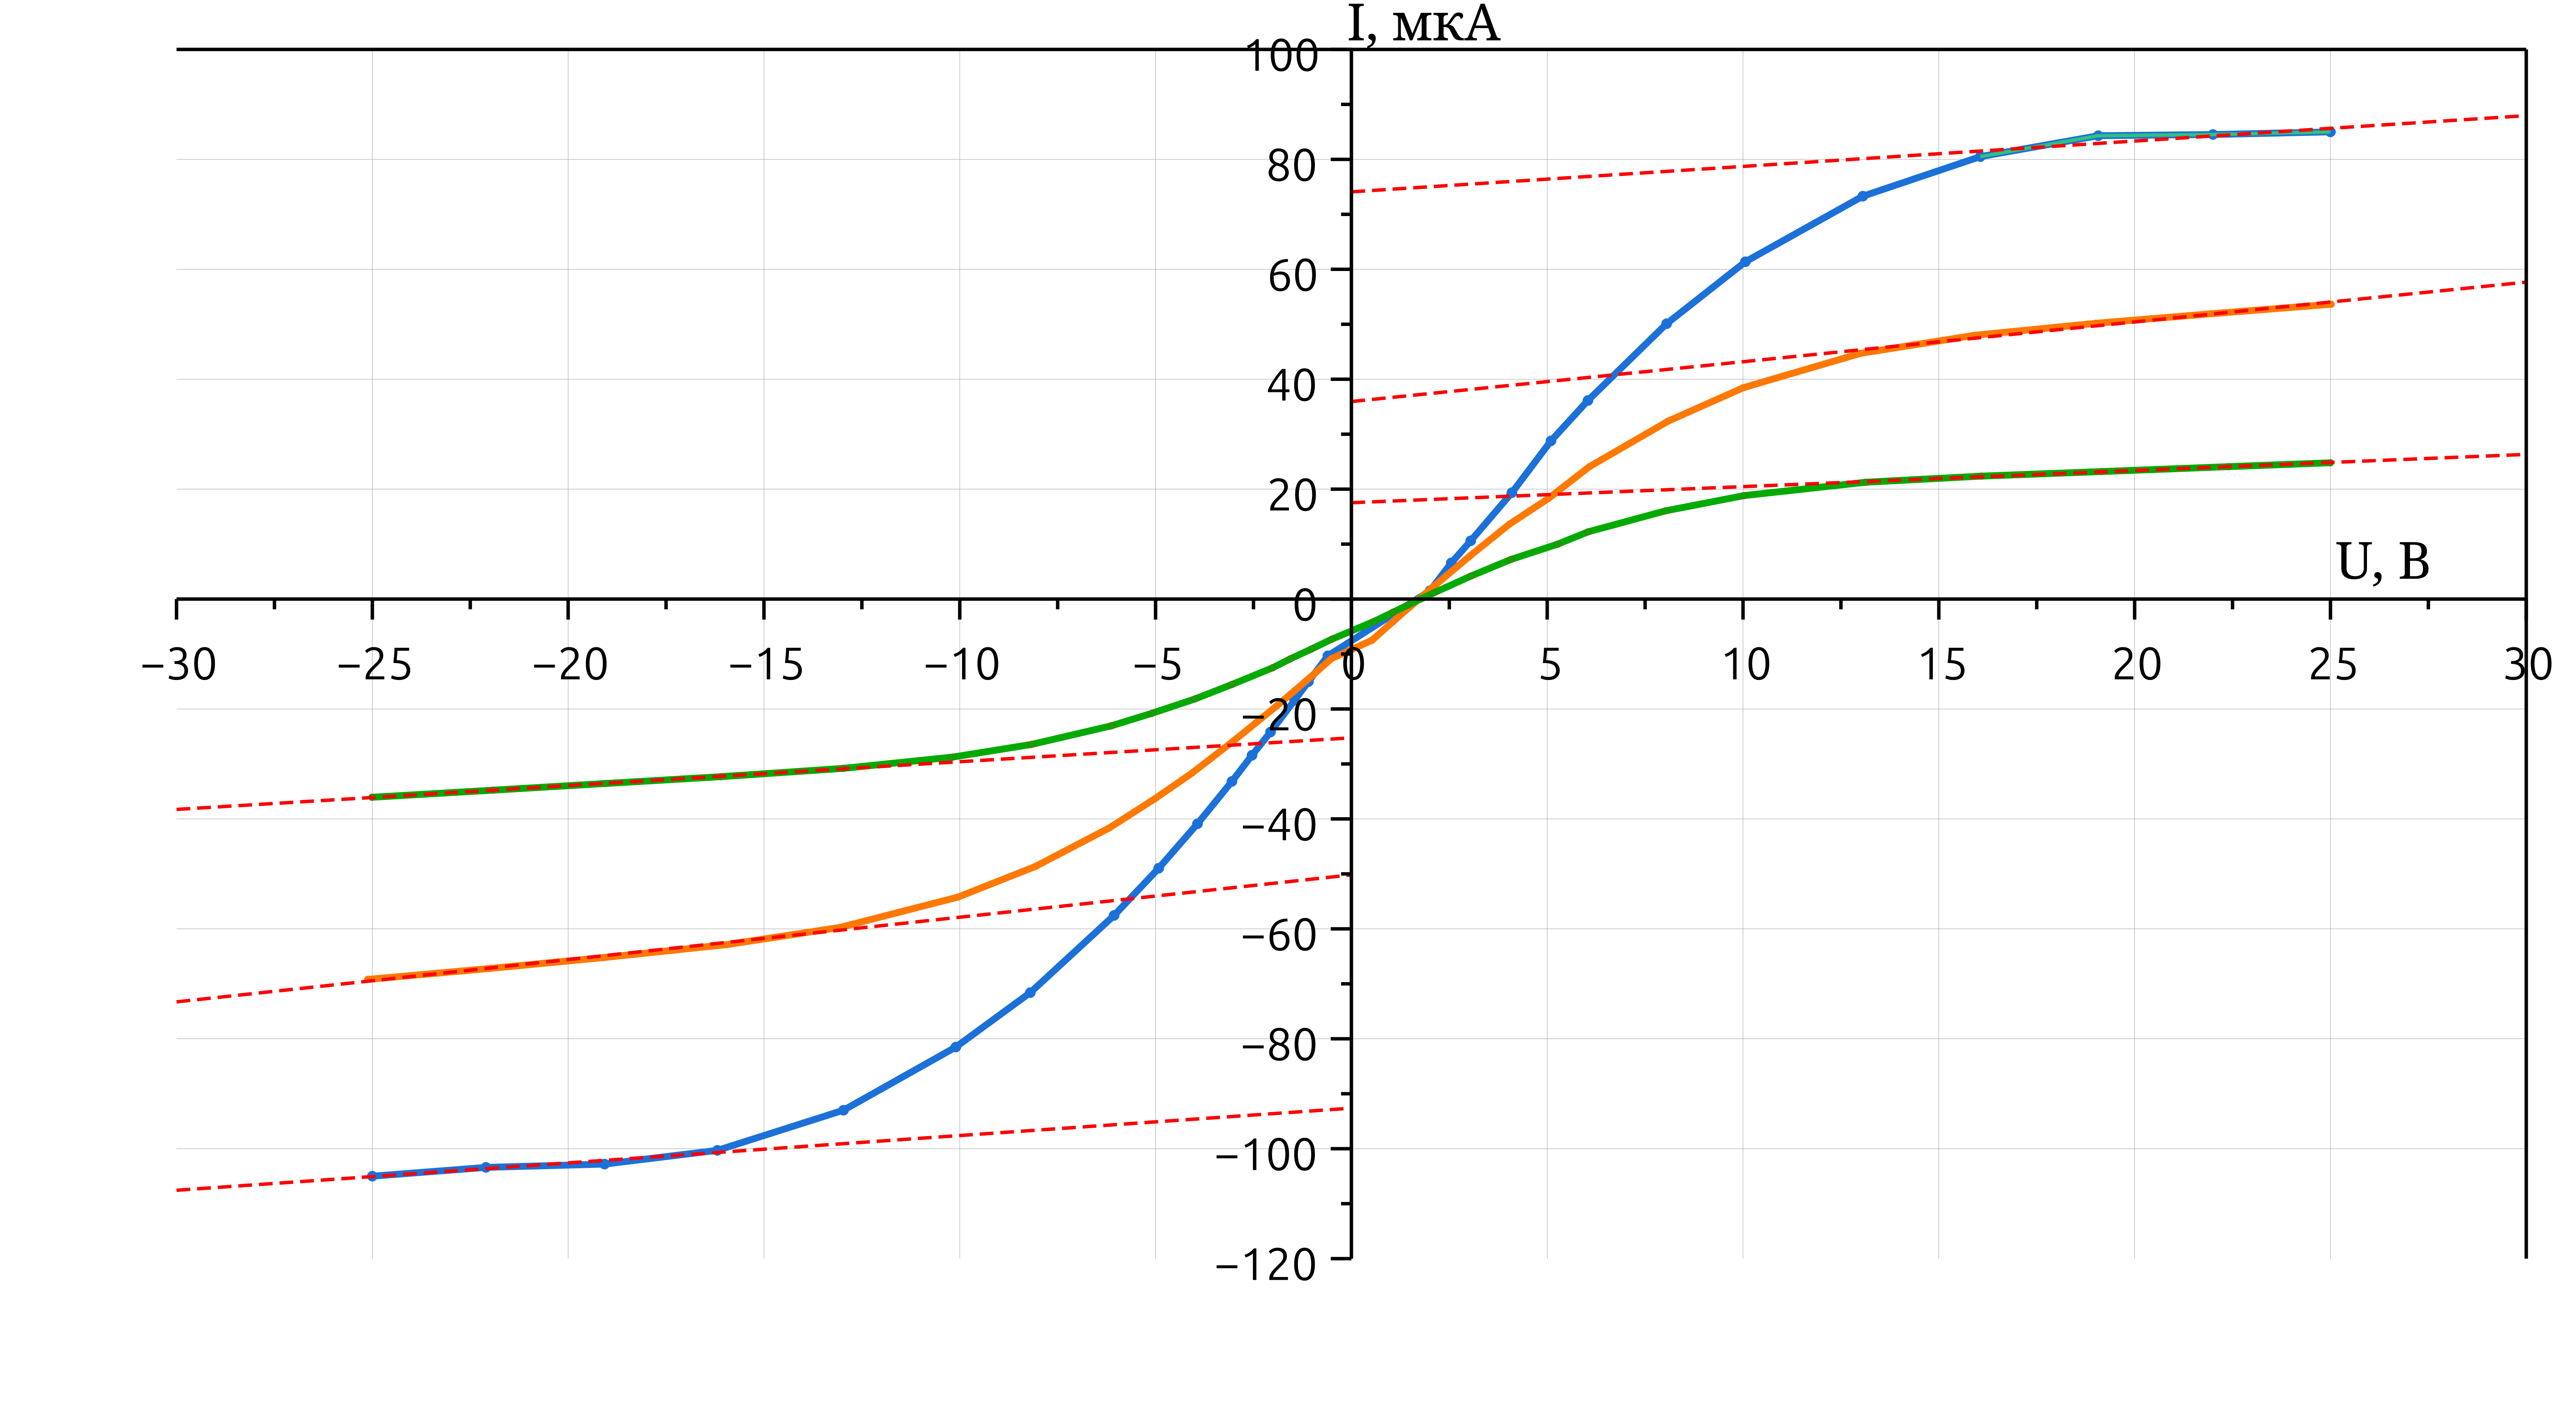
\includegraphics[width=\linewidth]{asymphota}
			\caption{ВАХ двойного зонда с проведёнными к ней касательными}
			\label{fig:all}
		\end{figure}
		
		
		
		
		\hspace{4.5mm} При трёх разных значениях тока разряда сняты вольт-амперные характеристики двойного зонда. Определены значения ионного тока насыщения по пересечению касательных к графикам при больших напряжениях с осью ординат (см. рис. \ref{fig:all}). Дифференцированием найден наклон характеристики вблизи начала координат(см. рис. \ref{fig:der}). Полученные значения сведены в таблицу 1. 
		
		Погрешности цифровых вольт- и амперметров приняты равными единице последнего разряда:  $\delta U = 0,01$ В и $\delta I = 0,1$ мкА соответственно. Они гораздо меньше статистического отклонения для измеренных величин. Поэтому основной источник погрешности при измерении тока насыщения и наклона ВАХ -- статистический, связанный с усреднением по малому количеству соответствующих значений. 
		
		\begin{figure}[h!]
			\centering
			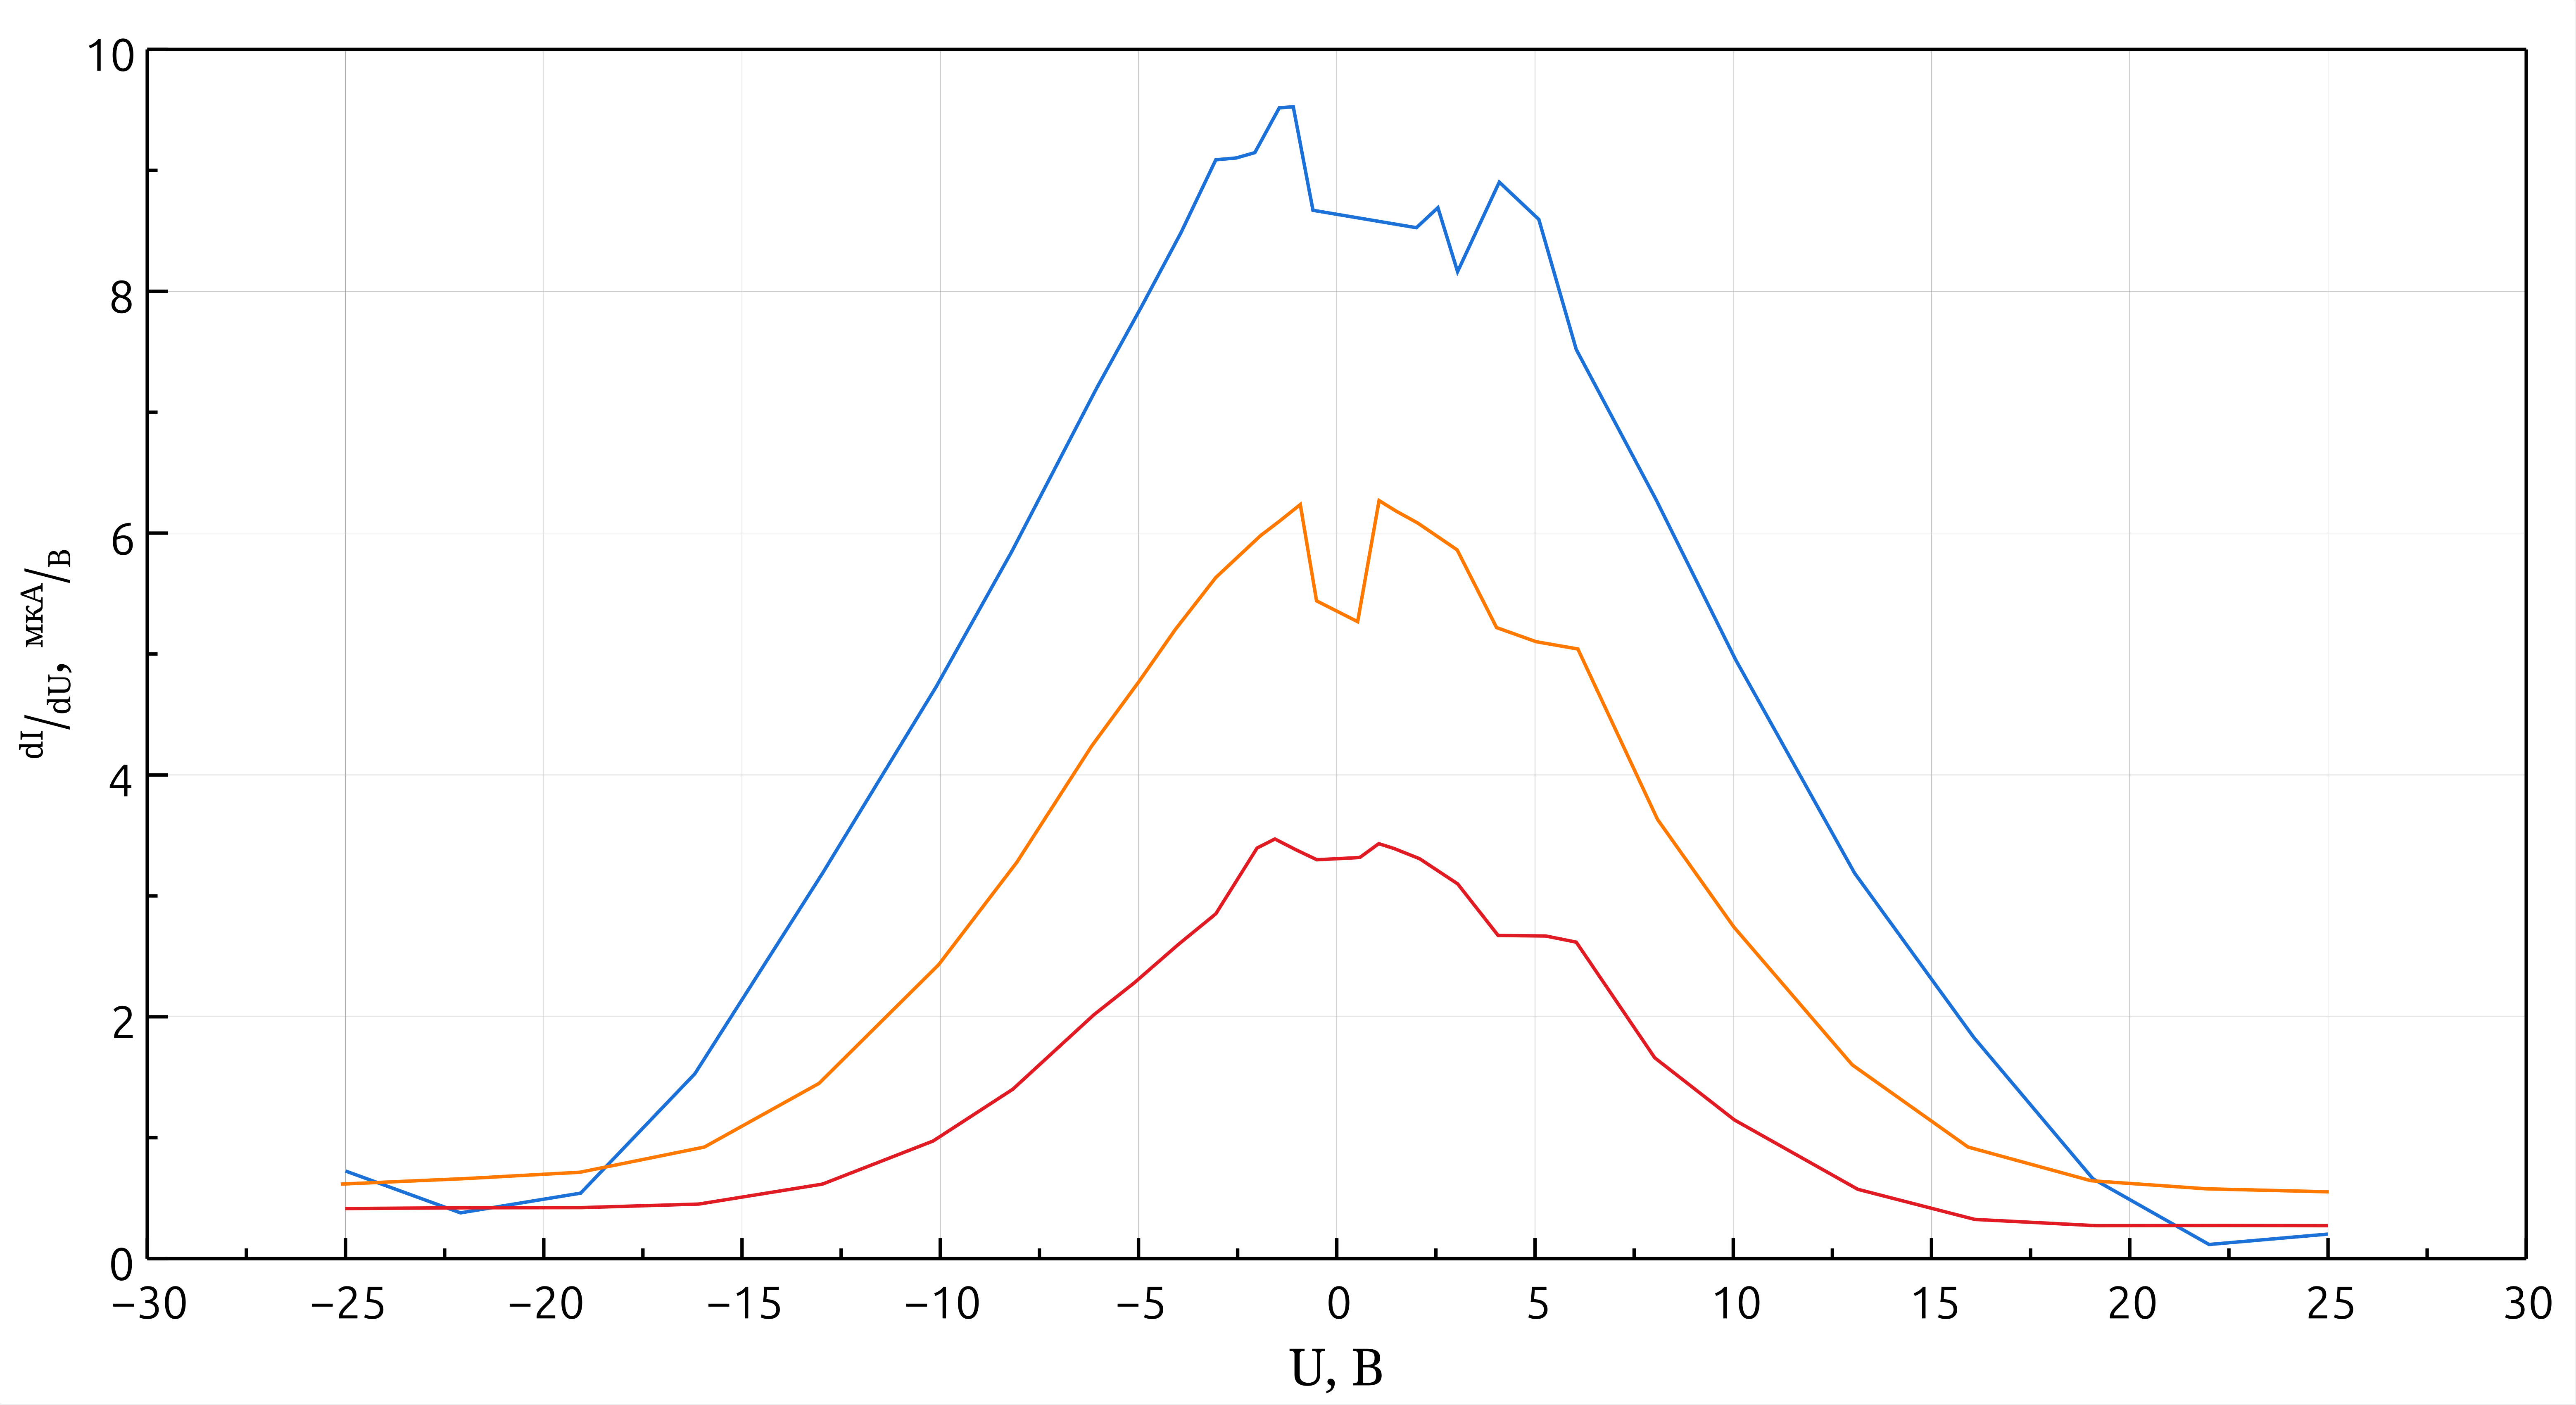
\includegraphics[width=0.5\linewidth]{der}
			\caption{Дифференцирование ВАХ двойных зондов}
			\label{fig:der}
		\end{figure}
		
		\begin{table}[h!]
			\caption{Зондовые характеристики}
			\centering
			\begin{tabular}{|r||c|c|c|}
				\hline
				Ток разряда, мА & 5 & 3 & 1,5 \\
				\hline
				Ионный ток насыщения, мкА & $83 \pm 2$ & $43,0 \pm 1,2$ & $21,4 \pm 0,5$\\
				\hline
				Наклон ВАХ вблизи нуля, мкА/В & $9,0 \pm 0,4$ & $5,9 \pm 0,4$ & $3,38 \pm 0,06$ \\
				\hline
				Температура электронов, эВ & $4,6 \pm 0,3$ & $3,6 \pm 0,3$ & $3,17 \pm 0,13$ \\
				\hline
				Концентрация ионов, м$^{-3}$ & $(6{,}3 \pm 0{,}5)\cdot10^{16}$ & $(3{,}7 \pm 0{,}3)\cdot10^{16}$ & $(1{,}9 \pm 0{,}2)\cdot10^{16}$ \\
				\hline
			\end{tabular}
		\end{table}
			
			\subsection{Параметры плазмы}
			
			\hspace{4.5mm}По найденным значениям $T_e$ и $n$ рассчитаны плазменная частота, дебаевские радиусы, число частиц в дебаевской сфере и степень ионизации. Результаты сведены в таблицу~\ref{tab:params}.
			
			\begin{table}
				\centering
				\caption{Параметры плазмы}
				\begin{tabular}{|l|c|c|c|}
					\hline
					Параметр & $I_p = 5$ мА & $I_p = 3$ мА & $I_p = 1{,}5$ мА \\
					\hline
					$T_e$, эВ & 4,6 & 3,6 & 3,17 \\
					$n$, $10^{10}$ см$^{-3}$ & $6{,}3$ & $3{,}7$ & $1{,}9$ \\
					$\omega_p$, $10^{9}$ рад/с & $14$ & $11$ & $7{,}8$ \\
					$r_{De}$, мкм & $64$ & $74$ & $95$ \\
					$r_D$, мкм & $4{,}8$ & $6{,}2$ & $8{,}6$ \\
					$N_D$ & 29 & 22 & 16 \\
					$\alpha$, $10^{-7}$ & $9{,}7$ & $5{,}7$ & $3{,}0$ \\
					\hline
				\end{tabular}
				\label{tab:params}
			\end{table}
			
			Плазма квазинейтральна: характерный размер трубки ($\sim10$ см) много больше $r_{De}$ ($\sim10^{-2}$ см). Число частиц в дебаевской сфере $N_D \gg 1$, поэтому плазму можно считать идеальной.
		
		
		


		
		
\section{Выводы}

	\hspace{4mm} В работе получена вольт-амперная характеристика тлеющего разряда в неоне в диапазоне напряжений 227--336 В. Показано, что ВАХ имеет отрицательный наклон и соответствует переходу от поднормального к нормальному тлеющему разряду. Дифференциальное сопротивление разряда лежит в пределах от $-65{,}8$ до $-6{,}6$ кОм.
	
	Методом двойного зонда измерены зондовые характеристики при трёх значениях тока разряда. Определены ионный ток насыщения, наклон ВАХ вблизи нуля и температура электронов. По формуле Бома найдена концентрация заряженных частиц. Вид и параметры ВАХ соответствуют теоретическим представлениям.
	
	Рассчитаны и другие параметры плазмы: плазменная частота, электронная поляризационная длина, дебаевский радиус экранирования, число частиц в дебаевской сфере, степень ионизации.
	
	Установлено, что плазма квазинейтральна ($L \gg r_{De}$) и идеальна ($N_D \gg 1$). С ростом тока разряда температура электронов падает, а концентрация растёт, что согласуется с теорией.
	
	Основной источник погрешности  в данной работе -- большой статистический разброс данных, превышающий все систематические погрешности измерений. Для уменьшения этого разброса можно брать больше экспериментальных точек на концах ВАХ и пересечении нуля.


\end {document}